\section{多层次图表示}
\label{sec:hcg}

\sys 使用 \graph 来描述张量程序在 GPU 上的执行。
\graph 包含多个层次的层次图，以在核（kernel）、块（block）和线程（thread）层次上表示计算\footnote{为简便起见，我们用{\em 块}（block）指代 CUDA 核的线程块（thread block），用{\em 线程}（thread）指代单个 CUDA 线程。}。
本节首先介绍 GPU 层次结构，并以 \Cref{fig:mugraph} 为运行示例，介绍 \graph 的关键组成部分。

\begin{figure}[t]
    \centering
    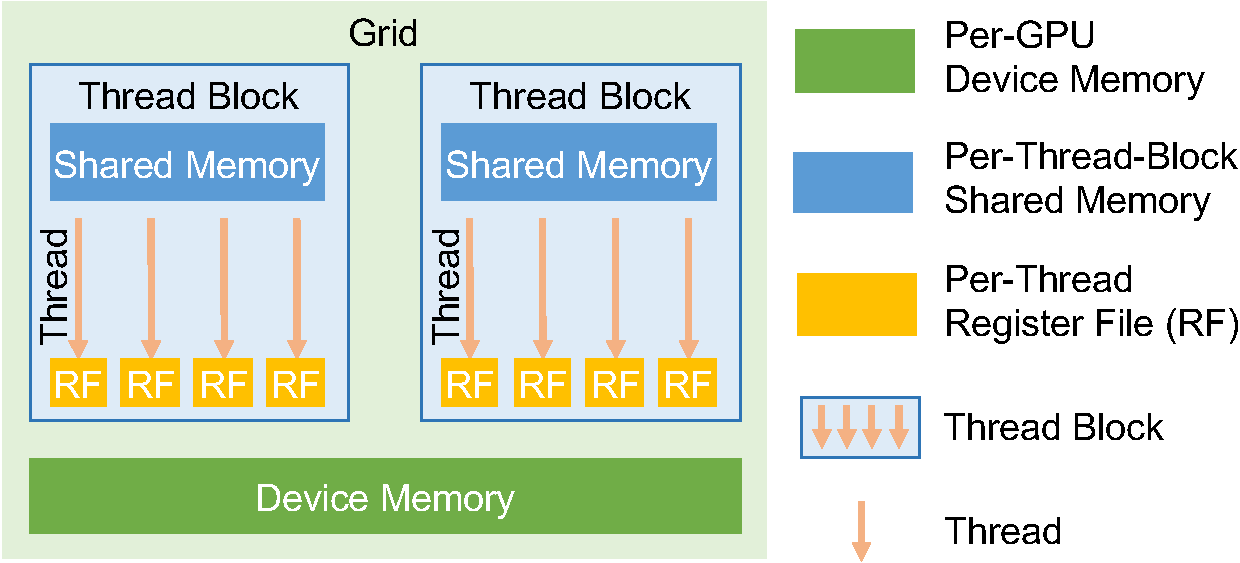
\includegraphics[width=\linewidth]{figs/gpu-hierarchy-crop.pdf}
    \caption{GPU 计算与内存层次结构。}
    \vspace{\captionvspace}
    \label{fig:gpu_hierarchy}
\end{figure}

\paragraph{GPU 层次结构。} \Cref{fig:gpu_hierarchy} 展示了当今 GPU 的层次结构。GPU 上的计算以{\em 核}（kernel）的形式组织，每个核是一个以单程序多数据（SPMD）方式在多个 GPU 核心上同时执行的函数。
一个核包含一个由{\em 线程块}（thread block）组成的网格，每个线程块在一个 GPU 流式多处理器上执行，并包含多个{\em 线程}（thread）来对各个数据元素执行计算。
每个线程关联一个线程私有的{\em 寄存器文件}（register file），同一线程块内的所有线程可以访问{\em 共享内存}（shared memory）以执行集体操作。
最后，核的所有输入和输出都存储在 GPU 的{\em 设备内存}（device memory）中。

\begin{figure}
    \subfloat[RMSNorm 与 MatMul 的计算图。] {
    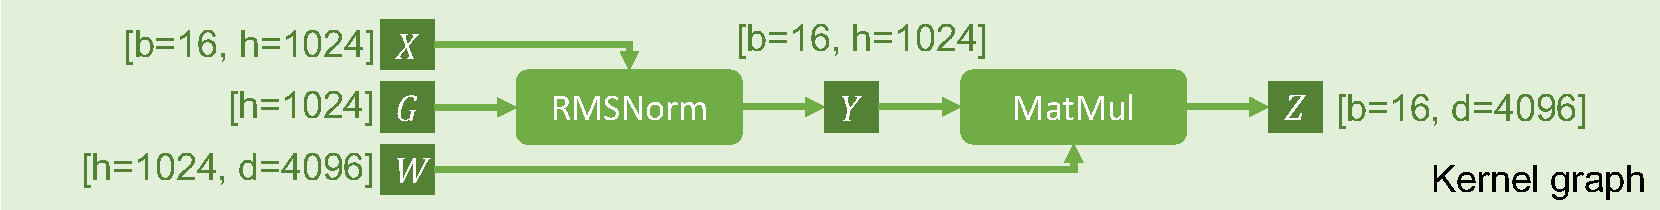
\includegraphics[scale=0.3]{figs/rms_norm_kernel_graph-crop.pdf}
    \label{fig:rms_norm_baseline}
    }
    \\
    \subfloat[\sys 发现的最优 \graph。]{
    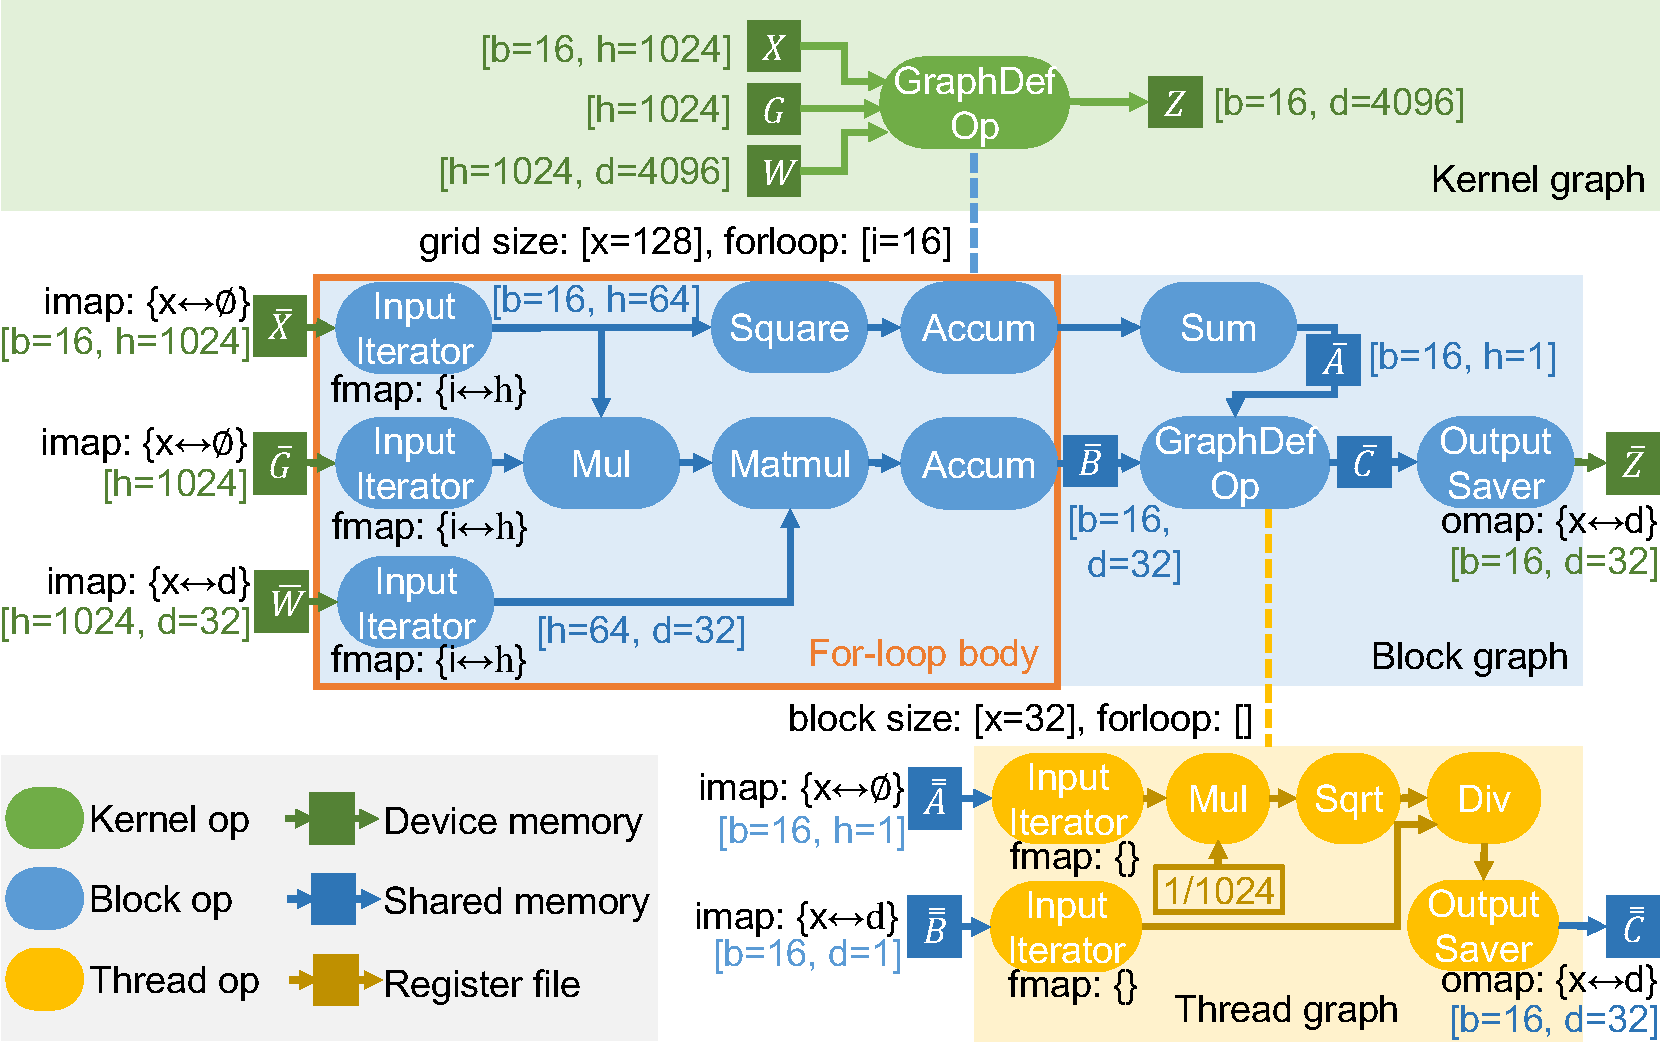
\includegraphics[scale=0.3]{figs/rms_norm_mugraph-crop.pdf}
    \label{fig:rms_norm_mlso}
    }
    \caption{\Cref{fig:rms_norm_baseline} 是 RMSNorm 与 MatMul 的计算图。\Cref{fig:rms_norm_mlso} 展示了 \sys 为计算 RMSNorm 和 MatMul 所发现的最优 \graph，该 \graph 将计算融合在单个核中以减少设备内存访问和核启动开销，比现有方法性能提升 $1.9\times$。括号中的数字表示张量形状，花括号中的数字显示对应运算符的 \imap、\omap 或 \fmap。}
    \vspace{\captionvspace}
    \label{fig:mugraph}
\end{figure}

\paragraph{核图（Kernel Graph）。}
每个张量程序对应一个{\em 核图}，其中每个节点代表运行在整个 GPU 上的一个核，每条边是核之间共享的张量。核图中的所有张量都存储在 GPU 设备内存中，因为不同的核无法在寄存器文件或共享内存中共享数据。
核图中的每个节点可以是{\em 预定义的}核运算符，由现有核库支持，例如 cuDNN~\cite{cudnn} 的卷积和 cuBLAS~\cite{cublas} 的矩阵乘法。
此外，为了支持细粒度的核间优化（如核融合），核图中的节点也可以是{\em 图定义的}核运算符，其语义和行为由一个更低层次（即块）图来定义。
例如，\Cref{fig:rms_norm_mlso} 中的核运算符就是一个由块图定义的图定义运算符。

\paragraph{块图（Block Graph）。}{\em 块图}描述与一个线程块相关的计算\footnote{在 CUDA 编程模型中，核的计算被定义为各独立线程块的计算。}，其中每个节点表示一个{\em 块运算符}，指定块内的计算，每条边（\Cref{fig:rms_norm_mlso} 中的蓝色箭头）是块运算符之间共享的张量。
\sys 出于以下两方面考虑，将块图中的所有中间张量存储在 GPU {\em 共享内存}中。
第一，GPU 共享内存比设备内存提供更高的带宽，这一设计使 \sys 能够通过最大限度地将中间结果保存在共享内存中来减少设备内存访问。
第二，对于大小超过共享内存容量而必须存储在设备内存中的张量，\sys 使用这些张量将计算拆分为多个块图，每个块图只包含共享内存中的张量，这种分离不会引入额外的设备内存访问。

每个块图还关联了描述其执行方式的属性，我们将在下面介绍。

\begin{figure}
    \centering
    \subfloat[$\er{imap} = \{x\leftrightarrow \er{column}\}$，$\er{fmap}=\{i\leftrightarrow \er{row}\}$]{
        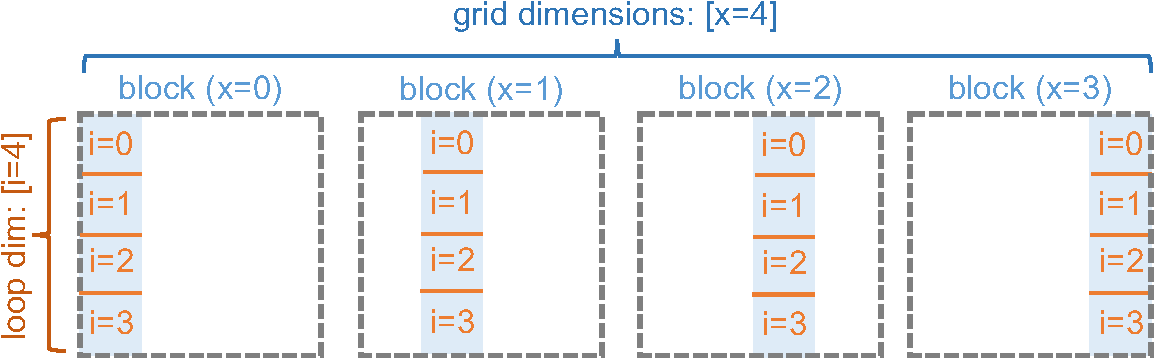
\includegraphics[scale=0.42]{figs/mapping_example_1_v2-crop.pdf}
    }
    \\
    \subfloat[$\er{imap}=\{x\leftrightarrow \phi, y\leftrightarrow \er{row}\}$，$\er{fmap}=\{i\leftrightarrow \er{column}\}$]{
        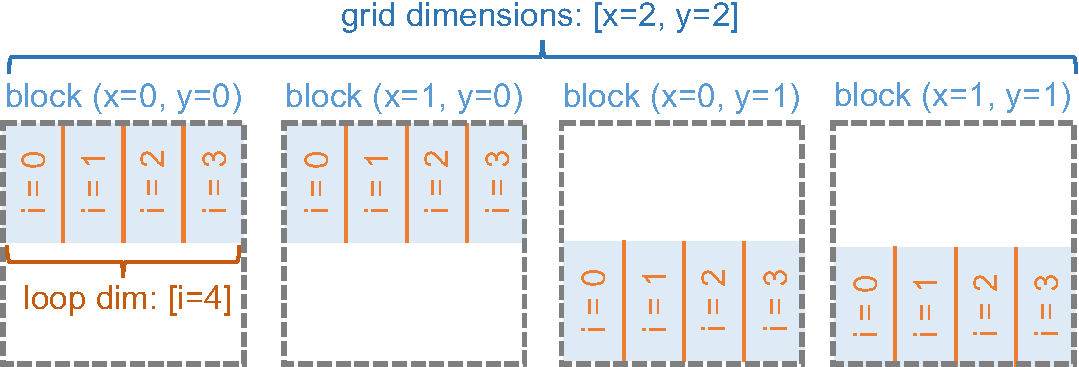
\includegraphics[scale=0.42]{figs/mapping_example_2_v2-crop.pdf}
    }
    \vspace{\captionvspace}
    \caption{演示如何使用 \imap 和 \fmap 将输入张量划分到各块和 for 循环迭代中。}
    \vspace{\captionvspace}
    \label{fig:mapping}
\end{figure}

\paragraph{网格维度（Grid Dimensions）。} 一个核内的所有块被组织成最多 3 维的网格，由 $x$、$y$ 和 $z$ 维来标识。块图关联最多三个{\em 网格维度}，指定 $x$、$y$ 和 $z$ 维上的块数。\Cref{fig:rms_norm_mlso} 中的块图启动了 $128$ 个块。

对于图定义核运算符的每个输入张量（例如 \Cref{fig:rms_norm_mlso} 中核图里的 $X$、$G$ 和 $W$），关联的块图包含一个 {\em \imap}，用于指定输入张量如何被划分为各个块的子张量。
对于每个网格维度（即 $x$、$y$ 或 $z$），\er{imap} 将其映射到（1）输入张量的某个数据维度，或（2）特殊的{\em 副本维度} $\phi$。
对于情况（1），映射的数据维度在该网格维度上的各块之间{\em 均等划分}；对于情况（2），输入张量在这些块之间{\em 复制}。
例如，\Cref{fig:rms_norm_mlso} 中的块图接收三个输入——$\overline{X}$、$\overline{G}$ 和 $\overline{W}$——代表每个块的输入张量。
对于 $\overline{W}$，其 $\imap=\{x\leftrightarrow d\}$ 表示张量 $W$ 的 $d$ 维被划分为 128 个等大小的块。因此，$\overline{W}$ 的形状为 $[h=1024, d=32]$。

其次，对于块图的每个输出张量（如 \Cref{fig:rms_norm_mlso} 中的 $\overline{Z}$），块图包含一个 {\em \omap}，指定如何将所有块的输出拼接以构建核运算符的最终输出。
在 \omap 中，每个网格维度必须映射到输出张量的某个数据维度，因为不同块必须在设备内存中存储不相交的张量。
对于 \Cref{fig:rms_norm_mlso} 中形状为 $[b=16, d=32]$ 的 $\overline{Z}$，其 $\omap =\{x\leftrightarrow d\}$ 表示具有相同 $x$ 索引的块沿 $d$ 维拼接，从而得到形状为 $[b=16, d=4096]$ 的张量 $Z$。

\paragraph{For 循环体。} 为了使大型输入张量能够放入共享内存，并将设备内存数据加载与计算重叠，块图可以包含一个 {\em for 循环体}，该循环体被反复执行以完成一个核的计算。
通常，核中的 for 循环之后会有一些后处理步骤。例如，计算平均值时，for 循环会对 $n$ 个值进行求和，而后处理步骤会除以 $n$。
\Sys 使用{\em 输入迭代器}（input iterators）、{\em for 循环累加器}（for-loop accumulators）以及二者之间的所有运算符来描述块图的 for 循环体（如 \Cref{fig:rms_norm_mlso} 中橙色框所示）。
块图的每个输入张量首先经过一个{\em 输入迭代器}，该迭代器将张量的一部分（如 $\overline{X}$、$\overline{G}$ 和 $\overline{W}$）从设备内存加载到共享内存中。
每个输入迭代器关联一个 {\em \fmap}，用于指定每次迭代中加载输入张量的哪个部分。形式上，\er{fmap} 将每个 for 循环维度映射到（1）输入张量的某个数据维度，或（2）副本维度 $\phi$。
与 \imap 类似，情况（1）时沿该维度均等划分，情况（2）时复制。
\Cref{fig:mapping} 展示了如何使用不同的 \imap 和 \fmap 将输入矩阵划分到各块和 for 循环迭代中。

每个块图还关联一个 {\em for 循环维度}，决定 for 循环体需要执行多少次以完成核的计算。此外，\sys 使用 {\em for 循环累加器}（如 \Cref{fig:rms_norm_mlso} 中的两个 {\tt Accum} 运算符）来累积每次迭代中计算的中间结果（使用标准累加器，如求和和取最大值），并将累积结果存储在共享内存中。for 循环体执行完毕后，\sys 继续直接对累积结果执行 for 循环体之外的其余运算符。{\em 输出保存器}（output saver）随后将共享内存中的最终结果保存回设备内存。

\paragraph{线程图（Thread Graph）。}{\em 线程图}进一步将计算范围从块缩小到单个线程。与块图类似，每个线程图也关联了{\em 块维度}（block dimensions，指定块内线程的组织方式）和 {\em for 循环维度}（for-loop dimensions，定义完成指定计算所需的总迭代次数）。每个线程图包含{\em 输入迭代器}（将输入张量从共享内存加载到寄存器文件中，如 \Cref{fig:rms_norm_mlso} 中的 $\overline{\overline{A}}$ 和 $\overline{\overline{B}}$）和{\em 输出保存器}（将输出张量从寄存器文件存储回共享内存，如 $\overline{\overline{C}}$）。
线程图是 \graph 中最低层次的图，只包含预定义的线程运算符。

\paragraph{张量布局（Tensor Layout）。}核图、块图或线程图中的每个张量都关联了一种{\em 张量布局}（为简便起见，\Cref{fig:mugraph} 中省略），用于指定张量在内存中的线性化方式。
注意，张量布局只影响 \graph 的性能，对输出的正确性没有影响。

\begin{definition}[\graph 合法性]
若一个 \graph $G$ 满足以下条件，则称其为{\em 合法的}：（1）对于 $G$ 中每个核、块和线程运算符 $o$，其输入和输出张量符合 $o$ 的规范；（2）每个核、块和线程图中的所有张量分别能够驻留在 GPU 的设备内存、共享内存和寄存器文件中；（3）对于每个含有 for 循环体的块图和线程图，从输入到输出的每条路径上恰好经过一个输入迭代器、一个 for 循环累加器和一个输出保存器。
\end{definition}

\paragraph{与先前工作的比较。}
先前工作分别考虑代数变换~\cite{TASO, wang2021pet}或调度变换~\cite{halide, tvm, autohalide}，而 \graphs 能够以统一的方式表示二者。
具体来说，网格维度和 for 循环维度及其对应的张量维度映射（即 \imap、\omap 和 \fmap）构成了图定义运算符可能调度的全面搜索空间。核、块和线程层次的层次图使得 \sys 能够在这些层次上探索代数变换。
